%-----------------------------------------------------------------------------------------------------------------------------------------------%
%	The MIT License (MIT)
%
%	Copyright (c) 2019 Jan Küster
%
%	Permission is hereby granted, free of charge, to any person obtaining a copy
%	of this software and associated documentation files (the "Software"), to deal
%	in the Software without restriction, including without limitation the rights
%	to use, copy, modify, merge, publish, distribute, sublicense, and/or sell
%	copies of the Software, and to permit persons to whom the Software is
%	furnished to do so, subject to the following conditions:
%	
%	THE SOFTWARE IS PROVIDED "AS IS", WITHOUT WARRANTY OF ANY KIND, EXPRESS OR
%	IMPLIED, INCLUDING BUT NOT LIMITED TO THE WARRANTIES OF MERCHANTABILITY,
%	FITNESS FOR A PARTICULAR PURPOSE AND NONINFRINGEMENT. IN NO EVENT SHALL THE
%	AUTHORS OR COPYRIGHT HOLDERS BE LIABLE FOR ANY CLAIM, DAMAGES OR OTHER
%	LIABILITY, WHETHER IN AN ACTION OF CONTRACT, TORT OR OTHERWISE, ARISING FROM,
%	OUT OF OR IN CONNECTION WITH THE SOFTWARE OR THE USE OR OTHER DEALINGS IN
%	THE SOFTWARE.
%	
%
%-----------------------------------------------------------------------------------------------------------------------------------------------%


%============================================================================%
%
%	DOCUMENT DEFINITION
%
%============================================================================%

%we use article class because we want to fully customize the page and don't use a cv template
\documentclass[10pt,A4]{article}	


%----------------------------------------------------------------------------------------
%	ENCODING
%----------------------------------------------------------------------------------------

% we use utf8 since we want to build from any machine
\usepackage[utf8]{inputenc}		

%----------------------------------------------------------------------------------------
%	LOGIC
%----------------------------------------------------------------------------------------

% provides \isempty test
\usepackage{xstring, xifthen}

%----------------------------------------------------------------------------------------
%	FONT BASICS
%----------------------------------------------------------------------------------------

% some tex-live fonts - choose your own

%\usepackage[defaultsans]{droidsans}
%\usepackage[default]{comfortaa}
%\usepackage{cmbright}
\usepackage[default]{raleway}
%\usepackage{fetamont}
%\usepackage[default]{gillius}
%\usepackage[light,math]{iwona}
%\usepackage[thin]{roboto} 

% set font default
\renewcommand*\familydefault{\sfdefault} 	
\usepackage[T1]{fontenc}

% more font size definitions
\usepackage{moresize}

%----------------------------------------------------------------------------------------
%	FONT AWESOME ICONS
%---------------------------------------------------------------------------------------- 

% include the fontawesome icon set
\usepackage{fontawesome}

% use to vertically center content
% credits to: http://tex.stackexchange.com/questions/7219/how-to-vertically-center-two-images-next-to-each-other
\newcommand{\vcenteredinclude}[1]{\begingroup
\setbox0=\hbox{\includegraphics{#1}}%
\parbox{\wd0}{\box0}\endgroup}

% use to vertically center content
% credits to: http://tex.stackexchange.com/questions/7219/how-to-vertically-center-two-images-next-to-each-other
\newcommand*{\vcenteredhbox}[1]{\begingroup
\setbox0=\hbox{#1}\parbox{\wd0}{\box0}\endgroup}

% icon shortcut
\newcommand{\icon}[3] { 							
	\makebox(#2, #2){\textcolor{maincol}{\csname fa#1\endcsname}}
}	

% icon with text shortcut
\newcommand{\icontext}[4]{ 						
	\vcenteredhbox{\icon{#1}{#2}{#3}}  \hspace{2pt}  \parbox{0.9\mpwidth}{\textcolor{#4}{#3}}
}

% icon with website url
\newcommand{\iconhref}[5]{ 						
    \vcenteredhbox{\icon{#1}{#2}{#5}}  \hspace{2pt} \href{#4}{\textcolor{#5}{#3}}
}

% icon with email link
\newcommand{\iconemail}[5]{ 						
    \vcenteredhbox{\icon{#1}{#2}{#5}}  \hspace{2pt} \href{mailto:#4}{\textcolor{#5}{#3}}
}

%----------------------------------------------------------------------------------------
%	PAGE LAYOUT  DEFINITIONS
%----------------------------------------------------------------------------------------

% page outer frames (debug-only)
% \usepackage{showframe}		

% we use paracol to display breakable two columns
\usepackage{paracol}

% define page styles using geometry
\usepackage[a4paper]{geometry}

% remove all possible margins
\geometry{top=1cm, bottom=1cm, left=1cm, right=1cm}

\usepackage{fancyhdr}
\pagestyle{empty}

% space between header and content
% \setlength{\headheight}{0pt}

% indentation is zero
\setlength{\parindent}{0mm}

%----------------------------------------------------------------------------------------
%	TABLE /ARRAY DEFINITIONS
%---------------------------------------------------------------------------------------- 

% extended aligning of tabular cells
\usepackage{array}

% custom column right-align with fixed width
% use like p{size} but via x{size}
\newcolumntype{x}[1]{%
>{\raggedleft\hspace{0pt}}p{#1}}%


%----------------------------------------------------------------------------------------
%	GRAPHICS DEFINITIONS
%---------------------------------------------------------------------------------------- 

%for header image
\usepackage{graphicx}

% use this for floating figures
% \usepackage{wrapfig}
% \usepackage{float}
% \floatstyle{boxed} 
% \restylefloat{figure}

%for drawing graphics		
\usepackage{tikz}				
\usetikzlibrary{shapes, backgrounds,mindmap, trees}

%----------------------------------------------------------------------------------------
%	Color DEFINITIONS
%---------------------------------------------------------------------------------------- 
\usepackage{transparent}
\usepackage{color}

% primary color
\definecolor{maincol}{HTML}{00a7e5}

% accent color, secondary
% \definecolor{accentcol}{RGB}{ 250, 150, 10 }

% dark color
\definecolor{darkcol}{RGB}{ 70, 70, 70 }

% light color
\definecolor{lightcol}{RGB}{245,245,245}


% Package for links, must be the last package used
\usepackage[hidelinks]{hyperref}

% returns minipage width minus two times \fboxsep
% to keep padding included in width calculations
% can also be used for other boxes / environments
\newcommand{\mpwidth}{\linewidth-\fboxsep-\fboxsep}
	


%============================================================================%
%
%	CV COMMANDS
%
%============================================================================%

%----------------------------------------------------------------------------------------
%	 CV LIST
%----------------------------------------------------------------------------------------

% renders a standard latex list but abstracts away the environment definition (begin/end)
\newcommand{\cvlist}[1] {
	\begin{itemize}{#1}\end{itemize}
}

%----------------------------------------------------------------------------------------
%	 CV TEXT
%----------------------------------------------------------------------------------------

% base class to wrap any text based stuff here. Renders like a paragraph.
% Allows complex commands to be passed, too.
% param 1: *any
\newcommand{\cvtext}[1] {
	\begin{tabular*}{1\mpwidth}{p{0.98\mpwidth}}
		\parbox{1\mpwidth}{#1}
	\end{tabular*}
}

%----------------------------------------------------------------------------------------
%	CV SECTION
%----------------------------------------------------------------------------------------

% Renders a a CV section headline with a nice underline in main color.
% param 1: section title
\newcommand{\cvsection}[1] {
	\vspace{14pt}
	\cvtext{
		\textbf{\LARGE{\textcolor{darkcol}{\uppercase{#1}}}}\\[-4pt]
		\textcolor{maincol}{ \rule{0.1\textwidth}{2pt} } \\
	}
}

%----------------------------------------------------------------------------------------
%	META SKILL
%----------------------------------------------------------------------------------------

% Renders a progress-bar to indicate a certain skill in percent.
% param 1: name of the skill / tech / etc.
% param 2: level (for example in years)
% param 3: percent, values range from 0 to 1
\newcommand{\cvskill}[3] {
	\begin{tabular*}{1\mpwidth}{p{0.72\mpwidth}  r}
 		\textcolor{black}{\textbf{#1}} & \textcolor{maincol}{#2}\\
	\end{tabular*}%
	
	\hspace{4pt}
	\begin{tikzpicture}[scale=1,rounded corners=2pt,very thin]
		\fill [lightcol] (0,0) rectangle (1\mpwidth, 0.15);
		\fill [maincol] (0,0) rectangle (#3\mpwidth, 0.15);
  	\end{tikzpicture}%
}


%----------------------------------------------------------------------------------------
%	 CV EVENT
%----------------------------------------------------------------------------------------

% Renders a table and a paragraph (cvtext) wrapped in a parbox (to ensure minimum content
% is glued together when a pagebreak appears).
% Additional Information can be passed in text or list form (or other environments).
% the work you did
% param 1: time-frame i.e. Sep 14 - Jan 15 etc.
% param 2:	 event name (job position etc.)
% param 3: Customer, Employer, Industry
% param 4: Short description
% param 5: work done (optional)
% param 6: technologies include (optional)
% param 7: achievements (optional)
\newcommand{\cvevent}[7] {
	
	% we wrap this part in a parbox, so title and description are not separated on a pagebreak
	% if you need more control on page breaks, remove the parbox
	\parbox{\mpwidth}{
		\begin{tabular*}{1\mpwidth}{p{0.72\mpwidth}  r}
	 		\textcolor{black}{\textbf{#2}} & \colorbox{maincol}{\makebox[0.35\mpwidth]{\textcolor{white}{#1}}} \\
			\textcolor{maincol}{\textbf{#3}} & \\
		\end{tabular*}\\[8pt]
	
		\ifthenelse{\isempty{#4}}{}{
			\cvtext{#4}\\
		}
	}

	\ifthenelse{\isempty{#5}}{}{
		\vspace{9pt}
		{#5}
	}

	\ifthenelse{\isempty{#6}}{}{
		\vspace{9pt}
		\cvtext{\textbf{Technologies include:}}\\
		{#6}
	}

	\ifthenelse{\isempty{#7}}{}{
		\vspace{9pt}
		\cvtext{\textbf{Achievements include:}}\\
		{#7}
	}
	\vspace{14pt}
}

%----------------------------------------------------------------------------------------
%	 CV META EVENT
%----------------------------------------------------------------------------------------

% Renders a CV event on the sidebar
% param 1: title
% param 2: subtitle (optional)
% param 3: customer, employer, etc,. (optional)
% param 4: info text (optional)
\newcommand{\cvmetaevent}[4] {
	\textcolor{maincol} {\cvtext{\textbf{\begin{flushleft}#1\end{flushleft}}}}

	\ifthenelse{\isempty{#2}}{}{
	\textcolor{darkcol} {\cvtext{\textbf{#2}} }
	}

	\ifthenelse{\isempty{#3}}{}{
		\cvtext{{ \textcolor{darkcol} {#3} }}\\
	}

	\cvtext{#4}\\[14pt]
}

%---------------------------------------------------------------------------------------
%	QR CODE
%----------------------------------------------------------------------------------------

% Renders a qrcode image (centered, relative to the parentwidth)
% param 1: percent width, from 0 to 1
\newcommand{\cvqrcode}[1] {
	\begin{center}
		\includegraphics[width={#1}\mpwidth]{qrcode}
	\end{center}
}


%============================================================================%
%
%
%
%	DOCUMENT CONTENT
%
%
%
%============================================================================%
\begin{document}
\columnratio{0.31}
\setlength{\columnsep}{2.2em}
\setlength{\columnseprule}{4pt}
\colseprulecolor{lightcol}
\begin{paracol}{2}
\begin{leftcolumn}
%---------------------------------------------------------------------------------------
%	META IMAGE
%----------------------------------------------------------------------------------------
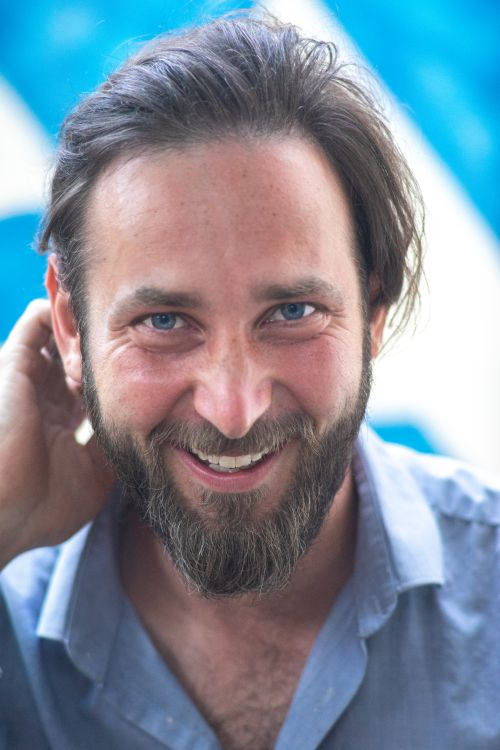
\includegraphics[width=\linewidth]{profile.jpg}	%trimming relative to image size

%---------------------------------------------------------------------------------------
%	META SKILLS
%----------------------------------------------------------------------------------------
\cvsection{MAIN IT SKILLS}

\cvskill{HTML/CSS/SASS/LESS} {17 yrs} {1} \\[-2pt]

\cvskill{Networking} {15 yrs} {0.8} \\[-2pt]

\cvskill{Linux} {15 yrs} {0.8} \\[-2pt]

\cvskill{Docker} {3 yrs} {0.7} \\[-2pt]

\cvskill{GIT} {10 yrs} {0.7} \\[-2pt]

\cvskill{HW (Building, Repairs)} {15 yrs} {0.6} \\[-2pt]

\cvskill{JavaScript, Python} {11 yrs} {0.6} \\[-2pt]

\cvskill{C, C++, Java, PHP} {10 yrs} {0.5} \\[-2pt]



\vfill\null
\cvsection{CONTACT}
	
\icontext{MapMarker}{12}{50 Sir John Young Crescent\\2011 Woolloomooloo, NSW}{black}\\[6pt]
\icontext{MobilePhone}{12}{+61 475 721 200}{black}\\[6pt]
\iconemail{Envelope}{12}{martin@knapovsky.com}{martin@knapovsky.com}{black}\\[6pt]

\vfill\null
%\cvqrcode{0.7}

%---------------------------------------------------------------------------------------
%	EDUCATION
%----------------------------------------------------------------------------------------
\newpage
\cvsection{EDUCATION}

\cvmetaevent
{2014 - 2017}
{Ing. in Cognitive Informatics}
{University of Economics, Prague}
{The primary goal of cognitive informatics is to develop computing systems that work best with how humans process information, creating more seamless human-systems integration. It is an interdisciplinary field that connects computer science, artificial intelligence, machine learning and interface design with human anatomy, physiology, neurology, psychology and philosophy.

In the master thesis a reverse engineering of Google search algorithms was done to show how to deliver accurate answer based on data collection about the user. 

Cognitive informatics was my major field of study, as a minor field I've chosen Philosophy where I've been studying about the theory of mind. The minor field of study was finished by a thesis concerning artificial intelligence and it's future implications. 
}

\cvmetaevent
{2008 - 2012}
{Bc. in Informatics}
{University of Technology, Brno}
{I've learned basics of many fields of IT - programming in languages like C, C++, Java, Python, Perl, using several types of databases, implementing algorithms, patterns, running simulations, rendering 3D graphics, analyzing voice, designing and testing interfaces, computer networking etc.
The topic of the bachelor's thesis was to create a 3D game that would run in a web browser and that would use a graphics card via WebGL technology.}

\vfill\null
%\cvqrcode{0.7}

%---------------------------------------------------------------------------------------
%	CERTIFICATION
%----------------------------------------------------------------------------------------
\newpage
\cvsection{CERTIFICATIONS}

\cvmetaevent
{CCNA Exploration: Network Fundamentals}
{}
{}
{}

\cvmetaevent
{CCNA Exploration: Routing Protocols and Concepts}
{}
{}
{}

\cvmetaevent
{CCNA Exploration: LAN Switching and Wireless}
{}
{}
{}


\cvmetaevent
{CCNA Exploration: Accessing the WAN}
{}
{}
{}

\cvmetaevent
{First Aid Certificate}
{}
{}
{}

\cvmetaevent
{EFR (Emergency First Response)}
{}
{}
{}

\cvmetaevent
{Driving License A2, B}
{}
{}
{}

\cvmetaevent
{TEFL - Teaching English as a foreign language}
{}
{}
{}

\cvmetaevent
{CAE - C1 Cambridge English}
{}
{}
{}

\cvmetaevent
{IELTS 8.5 English Certification}
{}
{}
{}

\vfill
%\cvqrcode{0.7}

\newpage
\mbox{} % hotfix to place qrcode on the bottom when there are not other elements
\vfill
%\cvqrcode{0.7}

\end{leftcolumn}
\begin{rightcolumn}
%---------------------------------------------------------------------------------------
%	TITLE  HEADER
%----------------------------------------------------------------------------------------
\fcolorbox{white}{darkcol}{\begin{minipage}[c][3.5cm][c]{1\mpwidth}
	\begin {center}
		\Huge{ \textbf{ \textcolor{white}{ \uppercase{ ING. MARTIN KNAPOVSKÝ } } } } \\[-20pt]
		\textcolor{white}{ \rule{0.1\textwidth}{1.25pt} } \\[4pt]
		\large{ \textcolor{white} {Freelance IT Consultant and Developer} }
	\end {center}
\end{minipage}} \\[14pt]
\vspace{-12pt}

%---------------------------------------------------------------------------------------
%	PROFILE
%----------------------------------------------------------------------------------------
\vfill\null
\cvsection{PROFILE}

\cvtext{32 years old IT consultant and developer with strong theoretical skills and a passion for open-source software and cloud services.\\

I'm specialized in working with Linux virtual private servers and deploying self-hosted cloud services for automation and a safe and private way to store personal/company data that is easily accessible to users from anywhere via a web browser or a mobile application.\\

Being originally from Czech Republic granted me the ability to speak Czech, although my main language has been English for past 4 years and I feel quite confident using this language in any kind of situation.

}

%---------------------------------------------------------------------------------------
%	WORK EXPERIENCE
%----------------------------------------------------------------------------------------
\vfill\null
\cvsection{WORK EXPERIENCE}

\cvevent
	{Feb 2017 - NOW}
	{IT Consultant and Developer}
	{Freelance}
	{As a freelancer, I've participated in several different roles. I'm using the skills I've learned in my previous jobs and studies and I'm combining them with my passion for photography and video. I can provide a complete online solution for small companies and individuals like server installation, hosting, web design, content creation or marketing.}
	{\cvlist{
		\item Deploying self-hosted cloud services like encrypted private email, cloud storage, git, private password manager, CRM, hosting, etc.
		\item System administration (linux)
		\item Building websites on top of Wordpress framework
		\item Logo design
		\item Marketing and SEO
		\item PC building, HW repairs
		\item Network infrastructure design and deployment
	}}
	{\cvlist {
		\item Docker, Kubernetes, Ansible, CapRover, Python, CSS, SASS, LESS, HTML5, JavaScript, GIT, PHP, Nginx, Jenkins
	}}
	{\cvlist{
		\item I'm able to offer an alternative solution to companies like Google, Microsoft or Apple for storing personal/company data privately and securely on their own infrastructure. 
		\item I've helped many businesses to promote themselves online and boost their revenue. 
		\item I've worked in various environments (AU, NZ, UK, Iceland, Malaysia, Indonesia, Czechia). 
	}}
	
	
\vfill\null
\cvevent
	{Sep 2015 - Feb 2017}
	{Research Assistant, University of Economics, Prague}
	{Management}
	{Administrative function at the university that I was studying.}
	{\cvlist{
		\item Communication with the Czech government
		\item University project management
		\item Coordination of student activities
		\item Maintenance of existing infrastructure
	}}
	{}
	{}

\vfill\null
\cvevent
	{Sep 2013 - Jan 2015}
	{Front-End Developer}
	{Webtoad.cz}
	{Responsible for design and implementation of user interfaces for custom web projects built on top of Nette framework.}
	{\cvlist{
		\item Selection of future-proof tools and infrastructure maintenance
		\item Design coding
		\item Quality assurance in terms of documentation
	}}
	{\cvlist {
		\item CSS, SASS, LESS, HTML5, JavaScript, GIT, PHP, Nginx, Jenkins
	}}
	{\cvlist{
		\item Working for international companies like Douwe Egberts and main Czech photography portal fotoaparat.cz.
	}}

\vfill\null
\cvevent
	{Jun 2013 - Jan 2014}
	{Front-End and Back-End Developer}
	{Webnaut.cz}
	{Building e-commerce websites on top of PrestaShop framework.}
	{\cvlist{
		\item Design and implementation of update and deployment process automaton
		\item Quality assurance by design of infrastructure monitoring, centralized logging solutions and documentation
	}}
	{\cvlist {
		\item PrestaShop Framework, PHP, HTML5, CSS, LESS, GIT, JavaScript
		\item Google Analytics
	}}
	{\cvlist{
		\item Custom reusable modules for PrestaShop
	}}

\vfill\null
\cvevent
	{Jun 2012 - May 2013}
	{Back-End Developer}
	{Nume.cz}
	{Building an auction portal for numismatics}
	{}
	{}
	{}
	
\vfill\null
\cvevent
	{Sep 2011 - May 2012}
	{3D Logical Game in Javascript}
	{Bachelor's thesis for Red Hat, Brno}
	{Developing a 3D clone of \textit{Berusky 3D} game on top of WebGL technology for running the game on-demand in a web browser}
	{}
	{}
	{\cvlist{
		\item 3D game accelerated on a graphics card running in a web browser that downloads it's updated data straight from the server and stores it in a local storage. 
	}}


% hotfixes to create fake-space to ensure the whole height is used
\mbox{}
\vfill
\mbox{}
\vfill
\mbox{}
\vfill
\mbox{}
\end{rightcolumn}
\end{paracol}
\end{document}